\newpage

\section{Proposed Research}
\label{sec:proposed-work}
The proposed research develops fast,
high-order-accurate, parallel numerical algorithms for large-scale
simulations of the collective hydrodynamics of amphiphilic particles in a viscous solvent.
%
We have demonstrated that our hydrophobic attraction with repulsion potential (HARP) approach efficiently simulates
self-assembly of amphiphilic particles into two-dimensional micelles, bilayer membranes, and vesicles \cite{Fu19}, and
recreates the tank-treading phenomenon in external shear flows \cite{Fu20}.
%
While the results show great promise in the field of collective body hydrodynamics,
several outstanding issues need to be addressed. These include a thorough 
analysis of elastic properties of our coarse-grained bilayers, and 
efficiently simulating three-dimensional collective hydrodynamics of amphiphilic particles.
Finally, we must mathematically characterize the variational behavior of HAP under appropriate homogenized limits.

\subsection{Specific Aim 1: Collective elastic and hydrodynamic properties of amphiphilic particles}
\label{subsec:specific_aim_1}

%\begin{figure}
%\begin{center}
%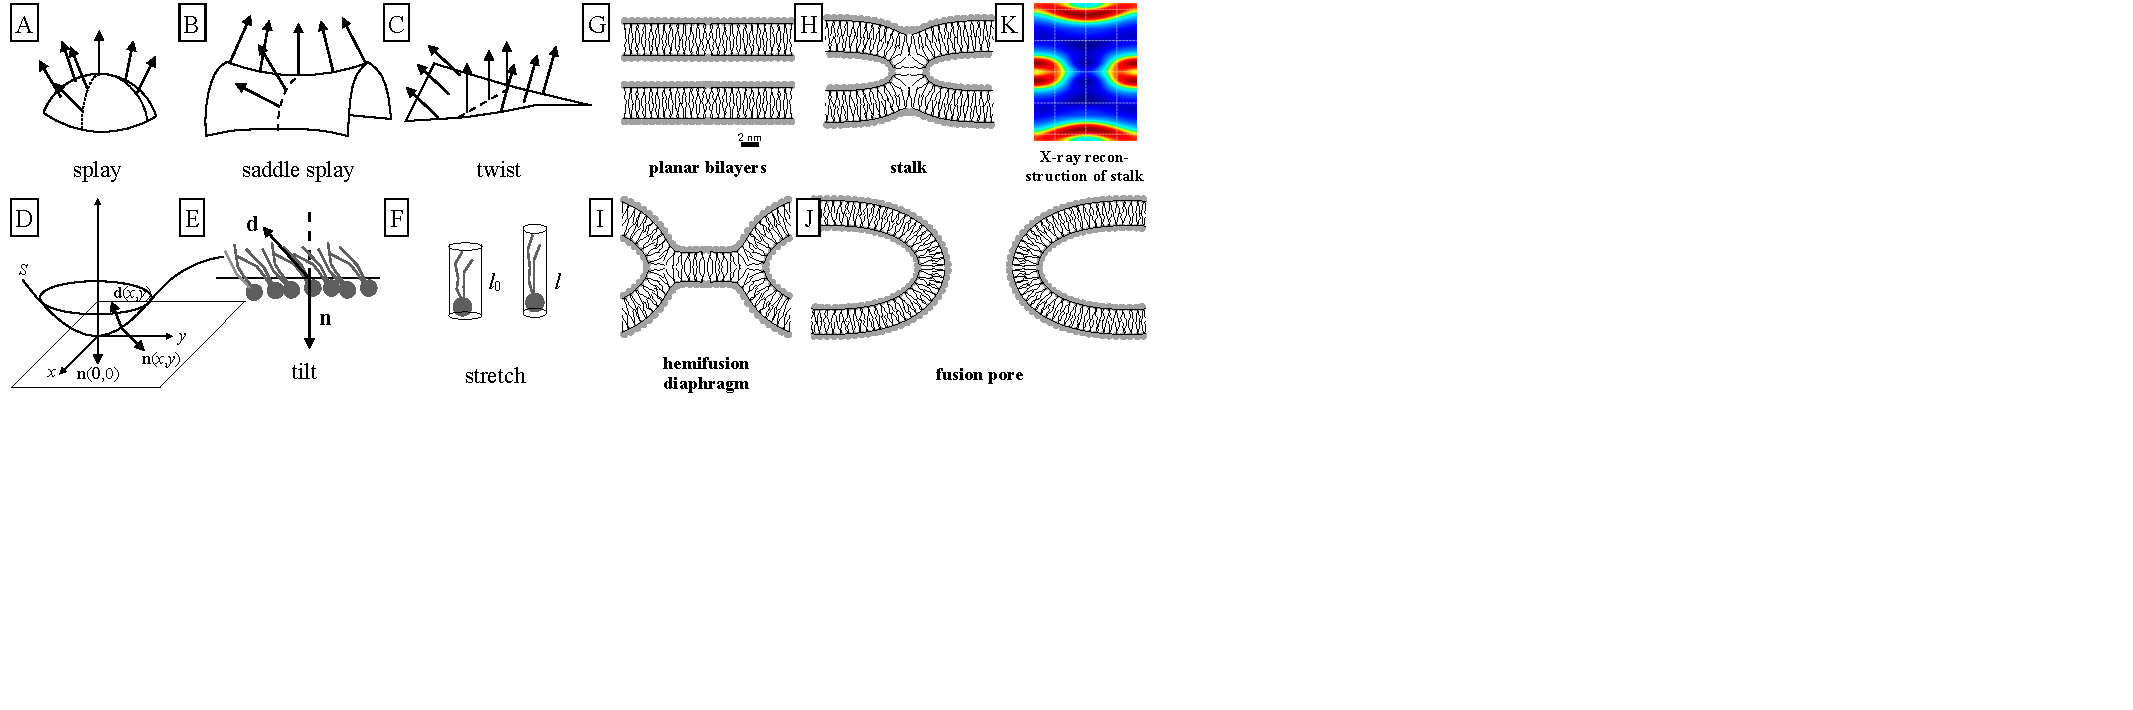
\includegraphics[width=0.9\textwidth]{figures/SA1_fig1.pdf}
%\end{center}
%\caption{\footnotesize (A--C) The splay ($\Div \mathbf{d}$), 
%saddle splay ($\det \mathsf{D}$) and twist ($\Curl \mathbf{d}$) elastic distortions of 
%a monolayer. (D) The monolayer neutral surface $\Sigma$,  
%director $\mathbf{d}$ and unit normal $\mathbf{n}$ in local coordinates.
%(E--F) Lipids are able to tilt from  the surface normal, and stretch.
%(H--J) Intermediates of membrane fusion and (K) experimental image of a stalk \cite{Aeffner2012}. }
%\label{fig:distortions}
%\end{figure}

The modern theory of membrane continuum mechanics
was pioneered by Hamm and Kozlov (HK) \cite{HaKo2000}.
The theory is widely used to describe biological phenomona 
fission \cite{10.1016/j.chemphyslip.2014.07.006, 10.1038/nature14509, 10.1103/PhysRevE.79.031926},
fusion \cite{10.1016/S0006-3495(02)75450-7,10.1073/pnas.121191898,10.1073/pnas.1119442109} ,
poration \cite{10.1016/j.bpj.2019.11.2221}, phase boundaries and interaction with inclusions
\cite{https://doi.org/10.1038/nrm.2017.16,10.1016/j.bpj.2019.11.2209, https://doi.org/10.1038/s41598-020-61110-2}, which require resolution of the internal structure of the membrane.  
%The Helfrich hamiltonian is widely used to determine energy barriers of fusion between lipid bilayer membranes \cite{ChKo08}. 
%Some of these barrier heights were never before obtained through the use of continuum membrane mechanics.
Using the HK  model as a base,
PI Ryham and collaborators calculated, for the first time in continuum theory, a least energy path for transitions between planar bilayers, a membrane stalk,
hemifusion diaphragm and the fusion pore \cite{RyWaCo13, RyKlYaCo16},
%The calculation of hydrophobic 
%fissures in \cite{RyKlYaCo16} motivated the HAP theory.
and the energies calculated by these continuum studies (Figure \ref{fig:barriers}A),
are in agreement with barrier heights derived by molecular dynamics and experimental studies \cite{FrRoPi17}.  
%analyzed the dependence of energy barriers on
%lipid composition and 

The HK framework assumes a three-dimensional, internal structure for lipid monolayers.
The internal structure consists of straight fibers that represent elongated hydrocarbon chains, and these fibers
tilt and stretch with respect to the dividing surface--the surface formed lying between the hydrocarbon chains and polar heads of lipids.
Accordingly, the deformation takes the form 
\begin{equation}
  \label{LMdeformation}
x(X_1, X_2, X_3) = x_0(X_1, X_2) + \zeta(x_0(X_1, X_2), X_3) n(x_0(X_1, X_2))
\end{equation}
where $(X_1,X_2,X_3)$ are points in a reference volume.
The map $x_0$ parametrizes the dividing surface $\Sigma$, and the unit vector field $n$ parametrizes the
direction of the lipid tails in the deformed state \cite{doi:10.1021/jp075641w,KLAUDA20083074}.
The parameter $X_3$ and the function $\zeta$ parametrizes the distance along the hydrocarbon chain in the reference state
and the deformed state, respectively, and so $0 \leq X_3 \leq \delta$ where $\delta \approx $ 2 nm is monolayer thickness. 

The elastic theory assumes an energy density that is quadratic in the Green-Lagrange strain tensor for $x$. 
The chains stretch and compress to satisfy incompressibility.
Symmetries with respect to mirror reflection and in-plane rotation, the internal structure assumptions and incompressibility
lead to an elastic surface energy over the dividing surface $\Sigma$. 
This energy decomposes into four, fundamental and independent deformations:
splay ($\Div n$), twist ($\Curl n$), saddle splay ($\det \nabla n$) and tilt $T$:
\begin{equation}
\label{ansatz3}
\begin{aligned}
\int_{\Sigma} 
  \tfrac{1}{2}\KB\left[ \left( \Div n + k_0\right)^2 - k_0^2\right] 
+ \tfrac{1}{2}\KT (\Curl n)^2 + \KG  \det \nabla n + \KTH |T|^2 \,dA.
\end{aligned}
\end{equation}
Here $\Div n$, $\Curl n$ and $\nabla n$ refer to the surface divergence, surface curl and surface gradient operators
respectively (Figure \ref{fig:distortions}A--C).
The deformations come with elastic coefficients: the \emph{bending modulus} $\KB$, \emph{twist modulus} $\KT$ 
and \emph{saddle-splay modulus} $\KG$ and \emph{tilt modulus} $\KTH$
HK define the tilt vector $T = n/(N\cdot n) - N$ where $N$ is the unit surface normal.

The parameter $k_0$ is the \emph{spontaneous curvature} and it determines the preferred lipid splay \cite{RoLi15,Kozlov2007}. 
As an illustration, the lipid DSPC has $k_0 = -0.1$ nm$^{-1}$ 
%as a result of  %having a relatively long acyl chain. 
and these lipids would line the  inner monolayer of a 
spherical liposome, because the addition of a positive splay $\Div \mathbf{d}$  in \eqref{ansatz3}
to the negative spontaneous curvature $k_0$ leads to lower energy \cite{Kamal22245, C3SM51829A, RoLi15,FriedSeguin15}.
The subtraction of $k_0^2$ makes the energy distortion free
\cite{Helfrich73,PhysRevLett.113.248102,Hamm2000}.

An interesting and challenging feature of \eqref{ansatz3} is that
the elastic energy couples director gradients to surface geometry through the tilt vector field.
In biological contexts, tilt appears at lipid domain boundaries, the edge of nanopores, and at the boundary of membrane inclusions \cite{https://doi.org/10.1103/PhysRevE.102.042406}, and the bilayer energy is the sum monolayer energies. 
Under spatial scales much larger than the membrane thickness, membrane energy is well-characterized by
the Canham-Helfrich energy used throughout the fluid-structure literature \cite{}.
The Canham-Helfrich energy is actually a special case of \eqref{ansatz3} obtained by setting $n =  \pm N$ (the $\pm$ depending
on orientation) and collapsing both monolayers onto the membrane midplane. There,
splay $\Div n$ equal to twice the mean curvature, saddle splay $\det \nabla n$ equal to the Gauss curvature,
and both twist and tilt equaling zero. 

The form of the elastic energy density \eqref{ansatz3} is the same as
the Oseen-Frank energy density for nematic liquid crystals \cite{ANDRIENKO2018520,Tran7106}.  In fact,  
a lipid monolayer acts as one layer in a smectic  phase \cite{REYESMATEO1995978,Rangamani20140463,PhysRevLett.113.248102}. 
The constants $\KB$, $\KT$  and $\KG$ play the same role as the Frank constants $K_1$, $K_2$ and $K_{24}$
liquid crystal theory. However, the ``bend'' distortion from nematics  
is not present in monolayers since the directors have no dependence in the normal direction.
There is also no ``spontaneous twist'' in monolayers due to invariance under mirror reflection. 

Recently, there has been a revival in interest in the HK theory. The quadratic assumption
for the elasticity energy density has caused researchers to question the validity of \eqref{ansatz}
for situations involving large curavtures \cite{PRL}. Zimmerberg and Akimov \cite{https://doi.org/10.1039/C9SM02079A}
showed that energies derived from molecular dynamics and elasticity agree even in the case of large deformations.
Part of this proposal will contribute to clarifying some of the mathematical
assumptions that went into the HK theory. 

%\begin{figure}
%\begin{center}
%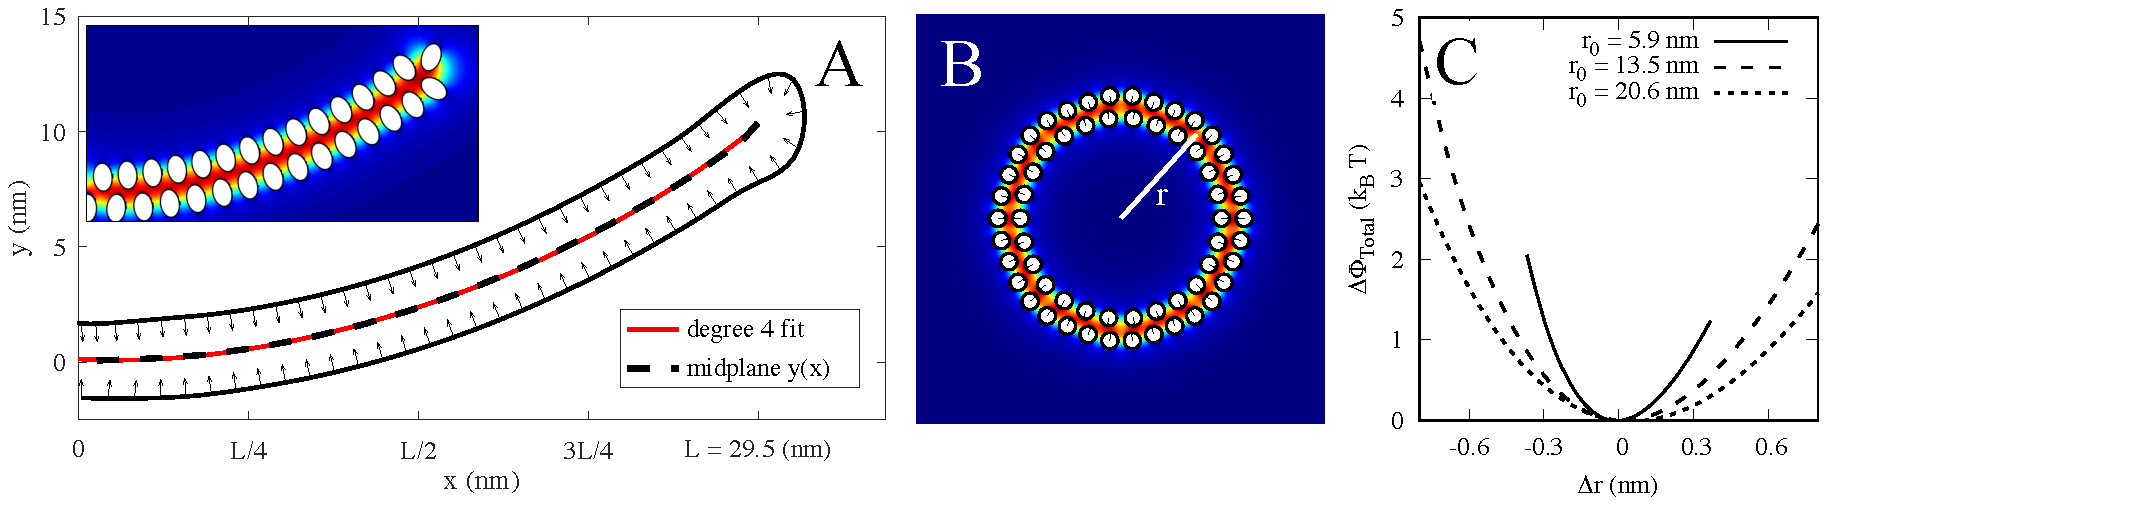
\includegraphics[width=\textwidth]{figures/SA1_fig2.pdf}
%\end{center}\vspace{-1.em}
%\caption{\footnotesize (A) A partially clamped bilayer with mid-plane (dashed curve) under uniform load.
%The quartic fit comes from continuum theory. 
%(B) A circular vesicle at equilibrium. (C) The area modulus derives
%from convexity in energy as a function of radius. 
%\label{fig:bend}}
%\end{figure}

\subsubsection{Evidence for elastic properties}
\label{sssec:evidence}
We tested for elastic properties by subjecting two-dimensional bilayer morphologies
to external loads \cite{Fu19}, using realistic
values for phospholipid length \cite{Boal},
the screening length $\rho = 2.5$ nm \cite{Eriksson1989,Lin2005,Parsegian,Israelachvili80,TerziDeserno17}
and  interfacial tension $\gamma=4.1$ pN nm$^{-1}$  \cite{GarciaSaez, KUZMIN2005, Petelska2012}.
Throughout the proposal, \kBT\; = 4.11$\times 10^{-21}$ J.
We first considered a planar bilayer subject to a uniform vertical load on the particle centers (Figure \ref{fig:bend}). 
The bilayer is clamped and horizontal at one end and the restoring force in the free part 
of the bilayer opposes the load. Twist and saddle splay are both zero, singling out splay
as the only distortion.
% In this situation, the directors are also parallel to the unit surface
%normal. As such $\Div \mathbf{d} = -2H$ where $H$ is the mean curvature of the surface. 
Since deformations are small \eqref{ansatz3}, it is possible to solve the bilayer loading in closed form. 
This analytical solution (red curve) basically overlaps the midplane of the particle based solution (Figure \ref{fig:bend}A). 

%\begin{wrapfigure}[13]{l}{0.5\textwidth}
%\centerline{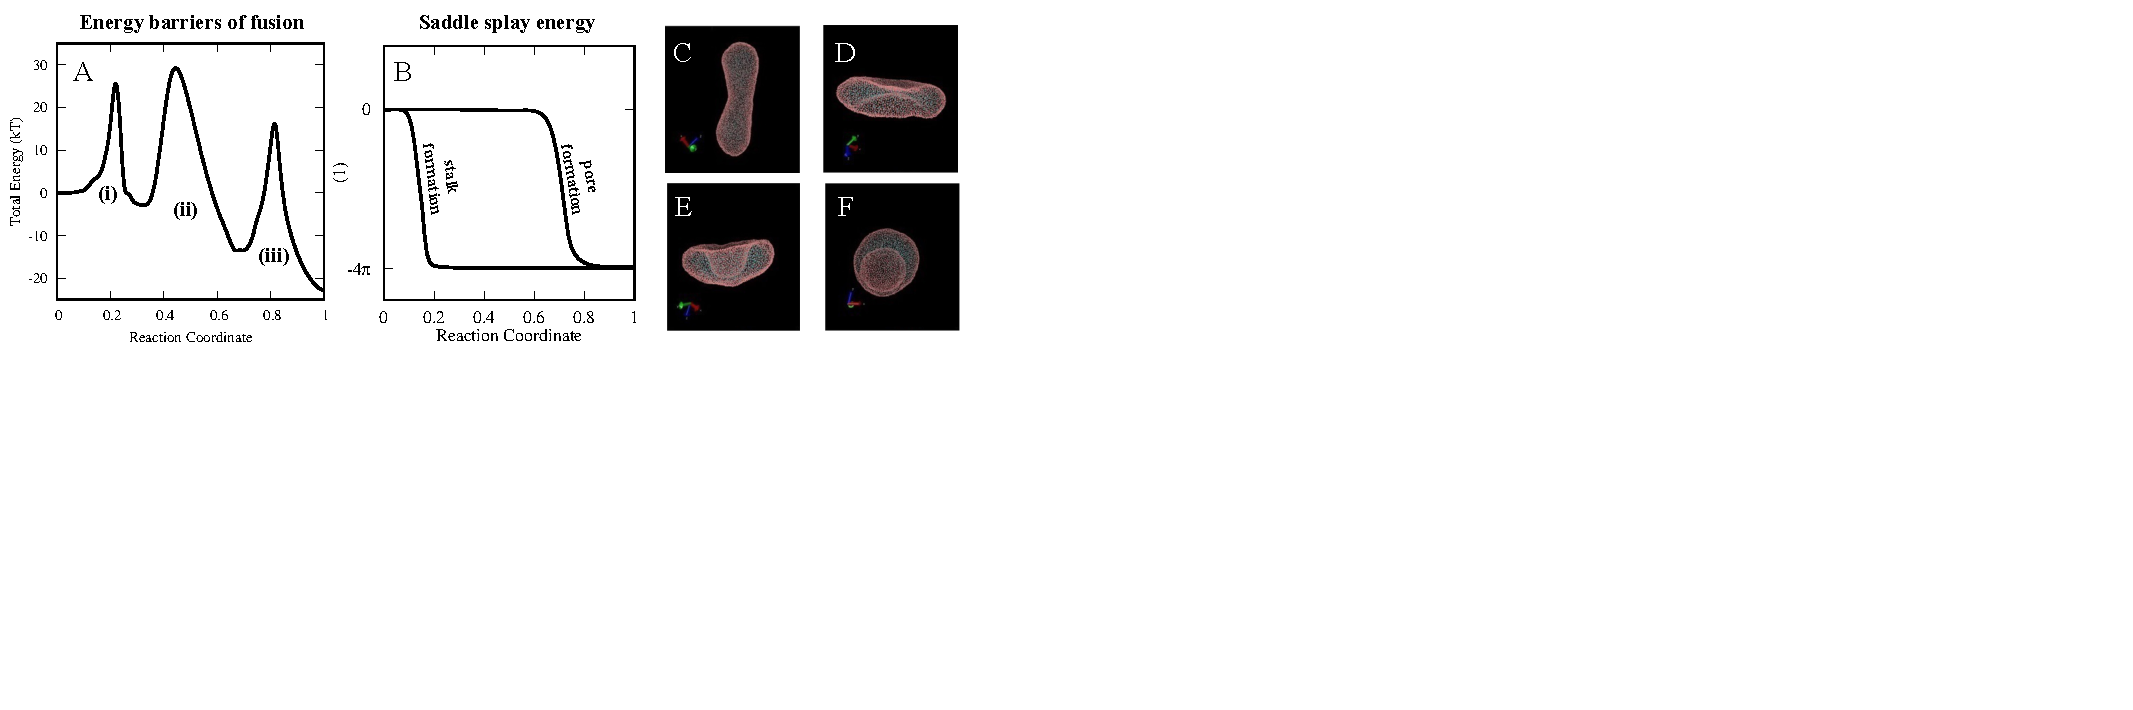
\includegraphics[width=0.5\textwidth]{figures/SA1_fig3.pdf}}
%\caption{{\footnotesize (A) Energy barriers for stalk formation (i), hemifusion
%diaphragm expansion (ii) and pore formation (iii). 
%(B) Saddle-splay energy for each change in \emph{monolayer} topology
%calculated in \cite{RyKlYaCo16}. (C)--(F): Shape transition of vesicle at different values of volume to area ratio from coarse-grained simulations of lipid bilayer membranes \cite{Fu16}.}}
%\label{fig:barriers}
%\end{wrapfigure}

Experimental measurements have accurately determined 
the bending modulus for several lipid types, with 
typical values lying around 10 \kBT\; \cite{Naetal15,VeBrPa15,NAGLE2000159,PhysRevLett.113.248102}.
By comparing with the exact solution, we derived a bending modulus
in the range 8.51 -- 13.54 \kBT, which is in 
excellent agreement with the experimentally derived value, especially considering how few parameters the HAP 
formalism involves. 

\newpage

\subsubsection{What work will actually be done?}
% Proposers should address what they want to do,
% why they want to do it,
% how they plan to do it,
% how they will know if they succeed,
% and what benefits could accrue if the project is successful.

We will study the elastic properties of particle-based bilayers using static and hydrodynamic, large particle-number simulation. 
The goal is to connect the deformations of particle bilayers to the deformations of HK theory, and in particular map the parameters of the
particle-based system onto known, and experimentally measured elastic moduli.

The successful outcomes of our preliminary tests suggest that the HAP particle configurations 
do behave like an elastic material. To validate our conjecture, we must consider 
ways to isolate or partially isolate the remaining distortions. 

\subsubsection{Hydrodynamic simulations}

\subsubsection{Static simulations}
Particle-based bilayers form because of the balance between hydrophobic attraction and excluded volume repulsion.
As a result, a precise way to measure a certain elastic properties is to set up an externally loaded system,
and then isolate the desired deformation by solving for the energy minimizer. The following give technical details on how we
draw these connections in practice.
In summary, the elastic moduli determine how lipid monolayers and bilayers mechanically behave.

\begin{description}
\item[Bending modulus] A planar bilayer that is deformed into the shape of a circular arc stores bending energy in the form of splay.
  Bending isolates the splay deformation $\Div{n}$ because the twist and saddle-splay deformations are zero in two-dimensional bilayers,
  and both MD and continuum mechanical simulations show that tilt is more or less zero due to lack of inclusions.
  Moreover, the splay in the two leaflets of an arc approximately cancel when added, due to the smaller head to tail ratio in the inner leaflet and
  larger head to tail ratio in the outer lealet, and so we can neglect the spontaneous curvature.

  Using steepest gradient descent, the simulation tracks the relaxation of the energies $E$ of a sequence of arc-shaped bilayers tending toward and the equilibrium, planar bilayer.
  We reconstruct the monolayer dividing surface (a curve $C$) and directors by interpolating the particle centers and orientations. Using spectral differentiation,
  we can compute the curvature $\kappa$ of $C$ and the squared curvature energy $H = \int_C \kappa^2$. Since $\Div{n} = -\kappa$ in this setup, we can plot
  the particle based values $\Delta E = E - E_0$ as a function of $\Delta H = H - H_0$ where $E_0$ and $H_0$ are the respective equilibrium values.

  Figure \ref{} shows the appoximately linear relationship between $\Delta E$ and $\Delta H$.
  The slope of the dashed line gives the bending modulus $\KB = 10$ kT. 
  The simulation is for a realistic phospholipid length \cite{Boal},
  the screening length $\rho = 2.5$ nm \cite{Eriksson1989,Lin2005,Parsegian,Israelachvili80,TerziDeserno17}
  and  interfacial tension $\gamma=4.1$ pN nm$^{-1}$  \cite{GarciaSaez, KUZMIN2005, Petelska2012}.

  The parameters of our hydrophobic attraction formalism map accurately onto the experimentally determined moduli.  
  The value $\KB = 10$ kT is a reasonable bending modulus for many lipid species \cite{}, and it depends linearly on
  the interfacial tension parameter $\gamma$ of our model. The $\gamma = 4.1$ pN nm$^{-1}$ is
  about a third of the surface tension of a typical hydrocarbon-water interface. M. Jackson points out, however, that the smaller interfacial tension parameter is actually the correct value 
  to describe the free energy for placing molecular lipid into contact with water \cite{}.
  So not only is the HARP model tunable to experimental parameters, but the results coincide with other properties from physical chemistry.  

\item[Tilt]
\item[Spontaneous curvature]
\item[Twist and saddle-splay]
  We measure the elastic response to twist by following the relaxation
  dynamics of an initially twisted membrane. Tilt is a fully three-dimensional deformation
  and so the reference membrane is a pancake-shaped, planar bilayer with diamater
  much larger than bilayer thickness.  In the initial configuration, the 
  the directors behave to leading order as $n = (0, mx_1, \sqrt{1 - m^2x_1^2})$
  where $x_1$ is the twisting axis. At the continuum level, 
  the surface gradient $\nabla n = \begin{pmatrix}0 & 0\\ m & 0\end{pmatrix}$ that $\Div n = \mathrm{tr}(\nabla n) = 0$,
  $\det(\nabla n) = 0$ and $\Curl d = (\nabla u)_{12} - (\nabla u)_{21} = m$,
  so that twist is isolated and the continuum elastic energy equals $\KA m^2 A + O(1)$ where
  $A \gg 1$ is the membrane area. 
  
  
  The initial bilayer consi
The twist deformation, for example, has a modulus in the range of 1 to 2 \kBT\; 
as evaluated by molecular dynamics \cite{LeVeWa14}. 
But twist is mathematically zero in our two-dimensional monolayers,
and so we require a computationally efficient means for evaluating the 
boundary integral equations in a collection of three-dimensional particles. 
Specific Aim 2 discusses some of the outstanding implementation issues. 

Our eventual three-dimensional calculations must also consider the saddle-splay distortion,
and the calculations may help resolve some well-known issues in the theory \cite{TerziDeserno17}. 
Theoretical analysis of lipid phase transitions predict a negative saddle-splay modulus around $-8$ \kBT\;
\cite{SIEGEL2004366,SIEGEL20085200}.
This value, however, 
predicts an energy barrier for monolayer fusion on the order of 200  \kBT, which runs counter to 
the value 30 \kBT\; estimated in experiments \cite{RyKlYaCo16,FrRoPi17,Tran7106}.  
We expect the particle-based approach can shed light on this inconsistency.   
\item[Stretching]
We also considered the stretching deformation \cite{Fu19}. 
Stretching occurs whenever there is an excess monolayer area,
and it is energetically costly since it exposes hydrocarbon tails to water. 
%Monolayers are not, strictly speaking, area incompressible,
%and 
Manipulation experiments give a monolayer area modulus in the range 
30 -- 40 \kBT\; nm$^{-2}$ \cite{Nagle17, Nagle17-2}. 
To measure an area modulus, we stretched a circular vesicle, modeling the cross-section 
of a bilayer tube (Figure \ref{fig:bend}B \& C).
%We then stretched the vesicle beyond and beneath equilibrium radius and recorded the change in energy. 
This procedure gave a monolayer area modulus 
34 $\pm$ 2 \kBT \;nm$^{-2}$, independently of the vesicle size, which
is also remarkably close to the experimental value.    


\item[Fluctuation spectrum]
\item[Revision of HK Theory]
  It may come as a surprise that the field of membrane continuum mechanics still lacks concensus as to
  whether \eqref{ansatz3} contains a complete list of consistent deformations.
  The PI Ryham showed, for example, that the tilt energy density is interchangagle, up to second order, with
  the simplified term $|n \times N|^2$ \cite{RyKlYaCo16}.
  Recently, \cite{10.1063/1.4990404} derived a tilt curvature term that Hamm and Kozlov had neglected from their analysis \cite{HaKo2000}.
  Later, \cite{https://doi.org/10.1039/C9SM02079A} 
  and \cite{10.1103/PhysRevE.102.042406} independently identified an inconsitency in the transversal tilt invariance
  assumption of Desrno's earlier work \cite{10.1063/1.4990404}.

  We suspect the reason why, after twenty years, the field has yet to reach a concensus 
  lies in the asymptotic expansions used to derive the elastic energy density. 
  Past researchers expressed the strain tensor in
  terms of the coordinate frame $\{\tau_1, \tau_2, N\}$ with surface tangent vectors $\tau_i$ and surface normal $N$.  
  In this frame, there is a coupling between the gradients of all three terms $x_0,$ $\zeta$ and $n$ of the deformation \eqref{LMdeformation}.
  The differential geometric arguments needed to determine which terms of the expansion to retain in the expansion are subtle,
  and have caused \cite{10.1103/PhysRevE.102.042406} to derive an energy density with more than ten elastic parameters, for example. 

  However, expanding the strain tensor in terms of the coordinate frame $\{e_1, e_2, n\}$ with $e_i$ perpendicular to $n$
  decouples a good portion of the gradient terms, leading to simplified expressions. For example,
  in this coordinate frame, the incompressility condition leads to an exact relationship 
  \begin{equation}
    \label{elongation}
    (1 + \Div n \zeta + \det \nabla n \zeta^2) \zeta' = 1
  \end{equation}
  for lipid elongation. \cite{HaKo2000} seem to have been aware of \eqref{elongation} for the special case of zero tilt,
  but the works \cite{HaKo2000, https://doi.org/10.1039/C9SM02079A, 10.1063/1.4990404} use an approximate form of \eqref{elongation}
  and \cite{10.1103/PhysRevE.102.042406} reports a form containing an erroneous $|T|^2$ in the $\zeta^0$ coefficient.   

Our investigations will leave open the possibility that the free energy of monolayers and bilayers is non-local. 
We have shown that hydrophic attraction is a non-additive force, meaning the force of attraction between two
particles is dependent on the position a third or more particles. Conceptually, this would arise in continuum theory if two monolayer surfaces
had different elastic energy density at that point despite having locally identical curvatures and directors.


\end{description}


\newpage
